\subsubsection{Overview}
Our puzzle system will be responsible for formally defining the nature and
functionality of the puzzles in our game.\\

The following diagram, Figure \ref{fig:puzzle_system_diagram}, gives a general overview
of the components of the puzzle system and how they communicate with one another.

\begin{figure}[!hb]
  \caption{Puzzle System Overview}
  \label{fig:puzzle_system_diagram}
  \centering
  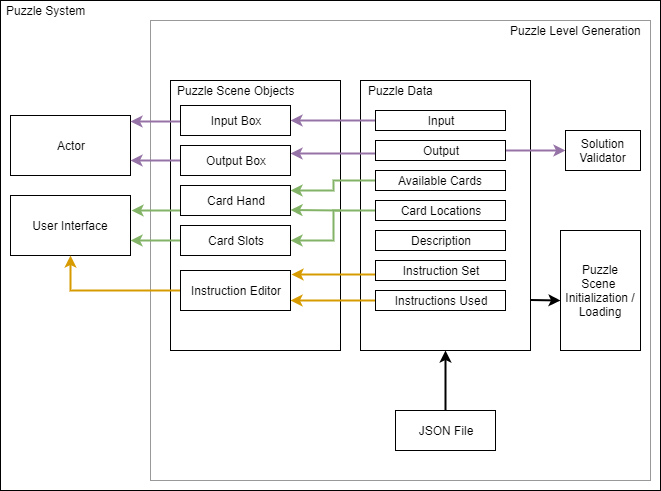
\includegraphics[scale=0.8]{Diagrams/puzzle_system_diagram.png}
\end{figure}
\vfill
\clearpage

The responsibilities of the puzzle system are as follows:

\begin{itemize}
	\item Present input to the player
	\item Determine the expected output the player is responsible for generating
	\item Offer allowed operations the player can perform to solve the puzzle
	\item Load an initial puzzle scene specific to each puzzle level
	\item Save a puzzle scene state for a specific level when the player leaves
	\item Load saved puzzle scene states for each level a player has previously attempted
\end{itemize}

Here are the main components of the Puzzle Scene that rely on the Puzzle System:

\begin{itemize}
	\item Input / Output (I/O)
	\begin{itemize}
		\item Input Box
		\item Output Box
		\item I/O Data (numbers)
	\end{itemize}

	\item Game Cards
	\begin{itemize}
		\item Player Card Hand
		\item Card Slots
	\end{itemize}

	\item Instruction Area
	\begin{itemize}
		\item Instruction bank
	\end{itemize}
\end{itemize}

Note that while the Game Cards and the Instruction Area fall under the User
Interface System, there are certain parts of these components that rely on
the Puzzle System’s level generation functionalities. Only that relationship
will be mentioned here. Refer to the User Interface System for a more detailed
look at these game components.

\subsubsection{Puzzle Level Generation}
When the player chooses a level, the puzzle system controls
which game objects get loaded in to the puzzle scene. This process is handled
by a puzzle generation script as seen in Figure \ref{fig:puzzle_level_data_flow}.\\

\begin{figure}[t]
  \caption{Puzzle Level Loading/Saving}
  \label{fig:puzzle_level_data_flow}
  \centering
  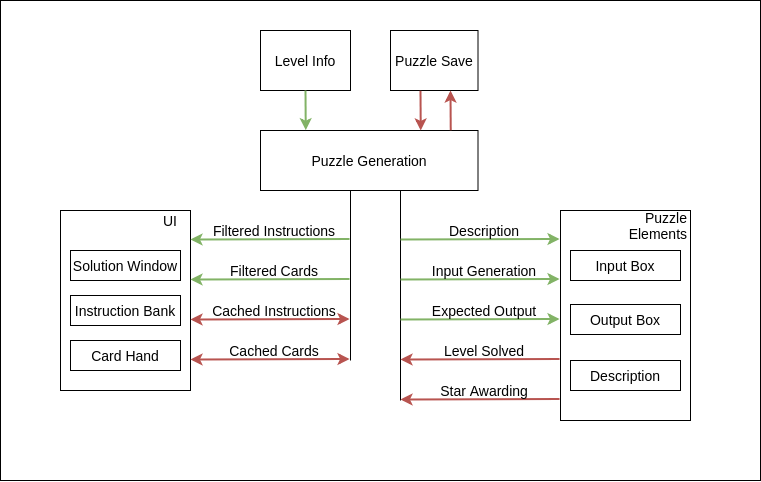
\includegraphics[scale=0.6]{Diagrams/PuzzleLevelDataFlow.png}
\end{figure}
\vfill

The puzzle generator uses two different kinds of data: initial puzzle data and saved puzzle data.\\

The initial puzzle data is the information that the scene will always need to load:
\begin{itemize}
  \item Input stream
  \item Expected output
  \item Level description
  \item Allowed instructions
  \item Allowed cards
  \item Number of each allowed card
  \item Hints
  \item Earnable awards
  \item Award requirements
\end{itemize}

This information varies from level to level. It is retrieved from a puzzle data script attached to
a game object that travels from a selected map node from the level selection scene. This can be
thought of as a base state of the puzzle level. If the player has never attempted the level, only
this data will be used when generating it.\\

Saved puzzle data is information that the puzzle generator needs to load from a previous attempt
at the puzzle level. It includes:
\begin{itemize}
  \item Instructions left in solution window
  \item Which instructions have been seen before
  \item Cards left in card played area
  \item Earned awards
  \item Was the puzzle solved
\end{itemize}

All of this data comes from a player state script which controls the player's save state that is in
use.

\subsubsection{Puzzle Level Caching}
When the player decides to leave a puzzle level (via exiting the game, returning to the
level menu, etc.), the puzzle system saves the state of the current level by using the player
state interface to write to the correct save file. This flow of information can be seen in
\ref{fig:puzzle_level_data_flow}.\\

All of the data that is saved is the same as the data that is loaded from previous puzzle attemps:
\begin{itemize}
  \item Instructions left in solution window
  \item Which instructions have been seen before
  \item Cards left in card played area
  \item Earned awards
  \item Was the puzzle solved
\end{itemize}

\subsubsection{Input}
The Puzzle System is in charge of filling the puzzle Scene's input box with data
that is necessary for the chosen level, shown by Figure \ref{fig:Puzzle_System_Input_Overview}.
The puzzle generator can either randomly generate an array of \textit{n} numbers or use a developer
specified input stream to fill the input box with corresponding data.\\

\begin{figure}[!hb]
  \caption{Puzzle System: Input Overview}
  \label{fig:Puzzle_System_Input_Overview}
  \centering
  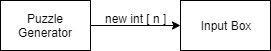
\includegraphics[scale=0.9]{Diagrams/Puzzle_System_Input_Overview.png}
\end{figure}
\vfill

The puzzle system is responsible for giving the Actor the correct data from the
input box when it is needed. The Actor can make an input request to the input box.
The system will simply return the top-most element from the input box to the Actor entity, along with the
numerical data that is associated with it behind the scenes (see Figure \ref{fig:Puzzle_System_Input_Actor}).\\

\begin{figure}[!hb]
  \caption{Input-Box/Actor Communication}
  \label{fig:Puzzle_System_Input_Actor}
  \centering
  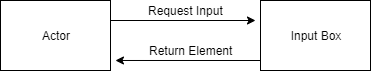
\includegraphics[scale=0.9]{Diagrams/Puzzle_System_Input_Actor.png}
\end{figure}

Note that if the Actor makes an input request to an empty input box, the puzzle system
will return NULL.\\

The input box has a fixed number of input items that can fit inside (5 in our examples).
Sometimes the size of the input stream can be larger than the size of the input box
itself. In this case, the input box works as a queue. If we had an input stream of
size six, the sixth element would be hidden until the top-most element of the input box
is removed by the Actor. All of the elements below will move up a slot and the
hidden sixth element would then appear at the bottom, as shown in Figure \ref{fig:Puzzle_System_Input_Overload_Before} and
Figure \ref{fig:Puzzle_System_Input_Overload_After}.\\

\begin{figure}[!htb]
  \caption{Input-Box Overloading (before)}
  \label{fig:Puzzle_System_Input_Overload_Before}
  \centering
  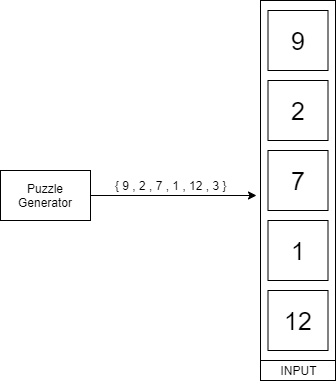
\includegraphics[scale=0.7]{Diagrams/Puzzle_System_Input_Overload_Before.png}
\end{figure}

\begin{figure}[!htb]
  \caption{Input-Box Overloading (after)}
  \label{fig:Puzzle_System_Input_Overload_After}
  \centering
  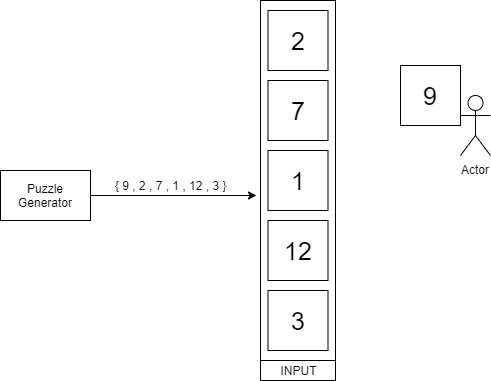
\includegraphics[scale=0.7]{Diagrams/Puzzle_System_Input_Overload_After.png}
\end{figure}
\vfill
\clearpage

If the input stream is the same size as the input box, or if the Actor has removed
enough numbers from a larger stream and there are no more slots to fill, the input numbers
behave only slightly differently. Figure \ref{fig:Puzzle_System_Input_Same_Before}
and Figure \ref{fig:Puzzle_System_Input_Same_After} show how the numbers below will move up a slot, like before,
but the bottom slot will be left empty.\\

\begin{figure}[!htb]
  \caption{Input-Box Same Size (before)}
  \label{fig:Puzzle_System_Input_Same_Before}
  \centering
  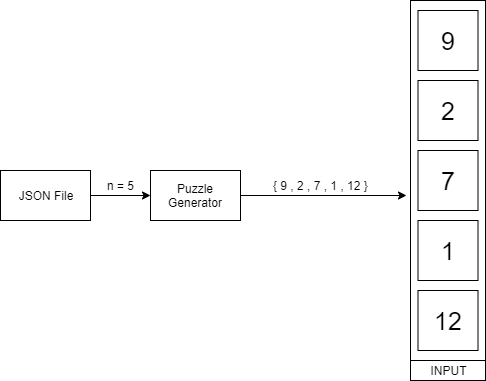
\includegraphics[scale=0.7]{Diagrams/Puzzle_System_Input_Same_Before.png}
\end{figure}

\begin{figure}[!htb]
  \caption{Input-Box Same Size (after)}
  \label{fig:Puzzle_System_Input_Same_After}
  \centering
  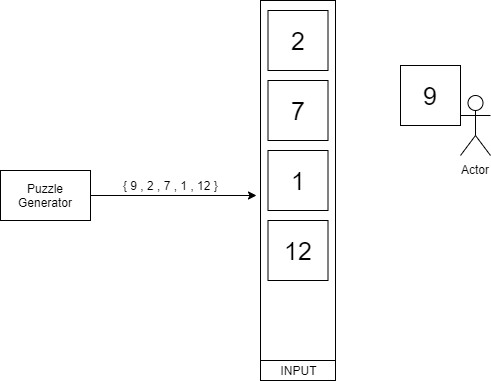
\includegraphics[scale=0.7]{Diagrams/Puzzle_System_Input_Same_After.png}
\end{figure}
\vfill
\clearpage

\subsubsection{Output}
In regards to output, the Puzzle System handles the interaction points between:
\begin{itemize}
  \item The output box
  \item The Actor
  \item The output validator
\end{itemize}
The Actor, after receiving an output instruction from the Interpreter, places the
data item from its hands to the output box. After all of the instructions are run, the
entire contents of the output box are submitted for validation, as shown in Figure
\ref{fig:Puzzle_System_Output_Interaction}.\\


\begin{figure}[!hb]
  \caption{Output Interaction Points}
  \label{fig:Puzzle_System_Output_Interaction}
  \centering
  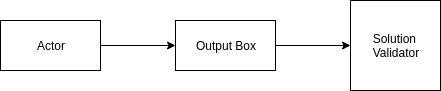
\includegraphics[scale=0.9]{Diagrams/Puzzle_System_Output_Interaction.png}
\end{figure}

A solution generation script generates the expected output based on the input that
was generated for that puzzle. An output validation script takes the contents of
the player's output box, their solution, and compares it against the expected output.
If the contents match, the player has solved the puzzle. If the contents do not match,
the player's solution did not solve the puzzle. The purpose for this confirmation of output
matching only is to allow the player to configure different algorithms that reach the same
solution, and inherently present a challenge to find the ideal solution to garner the best
possible score. Figure \ref{fig:Puzzle_System_Output_Validation} shows the decision process
of validating a solution.

\begin{figure}[t]
  \caption{Output Validation}
  \label{fig:Puzzle_System_Output_Validation}
  \centering
  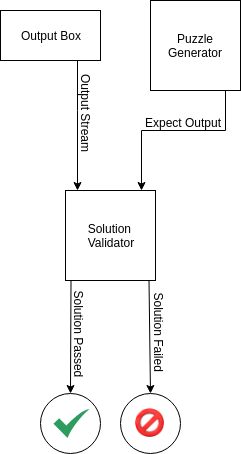
\includegraphics[scale=0.9]{Diagrams/Puzzle_System_Output_Validation.png}
\end{figure}
\vfill

\subsubsection{Game Cards}
The Puzzle System makes use of the puzzle generator in order to tell the user interface
which game cards are placed in certain positions on the game board when beginning
or loading a level. Allowed cards are retrieved from the current level's puzzle data object.
Card positions are pulled from the player state save file.
A card position not only indicates if a card is in the player's card hand or the puzzle board's
card slots, but also the position within either of those areas.\\

The card hand is filled during initialization. The puzzle data object will contain the following:
\begin{itemize}
   \item Number of register cards
   \item Number of stack cards
   \item Number of queue cards
   \item Number of heap cards
\end{itemize}

The initial content of the card hand is based on this data, although the locations
of these cards may be changed later on. Cards can move between two different puzzle scene areas:
\begin{itemize}
   \item Card hand area
   \item Card played area
\end{itemize}

Any update to a card's position will be reflected when returning to that level.
When a level is exited, all of the cards locations on the game board are saved to
that level's save file. When a level is loaded at another point in time, the card
objects will be instantiated like above, but also placed at their saved locations.\\

\subsubsection{Instructions}
The puzzle scene tells the instruction editor component of the User Interface:
\begin{itemize}
  \item Which instructions the player can use for the current level
  \begin{itemize}
    \item These will initially appear in the instruction bank
  \end{itemize}
  \item Which instructions were left in the editor during a previous attempt at
  the puzzle level
  \begin{itemize}
    \item These will appear where they were left in the editor previously
  \end{itemize}
\end{itemize}

The puzzle level's puzzle data object contains the information that the User Interface
needs to present the player with the appropriate instructions for a given puzzle level.
The puzzle generator reads the puzzle data and passes the instruction set off to the User Interface
as shown in Figure \ref{fig:Instruction_Flow}.

\begin{figure}[t]
  \caption{Loading Instruction Set}
  \label{fig:Instruction_Flow}
  \centering
  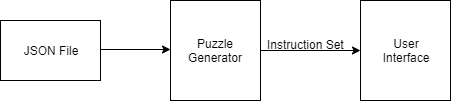
\includegraphics[scale=0.9]{Diagrams/Puzzle_System_Instruction_Flow.png}
\end{figure}

The player's save file tells the user interface which
instructions were left in the editor (Figure \ref{fig:Instruction_Flow2}). The initial state of the puzzle level leaves the
editor empty. Otherwise, the editor is populated with the same instructions that were
left during a previous attempt. This also includes final solutions that actually solved the
puzzle level.

\begin{figure}[!hb]
  \caption{Loading Instruction Editor State}
  \label{fig:Instruction_Flow2}
  \centering
  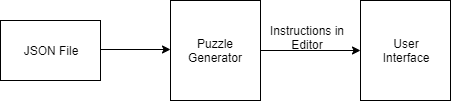
\includegraphics[scale=0.9]{Diagrams/Puzzle_System_Instruction_Flow2.png}
\end{figure}
